\documentclass[11pt,a4paper]{article}

% for Chinese
%\usepackage{fontspec}  % 加這個就可以設定字體
%\usepackage[BoldFont, SlantFont]{xeCJK}  % 讓中英文字體分開設置
%\setCJKmainfont{新細明體}  % 設定中文為系統上的字型,而英文不去更動,使用原TeX\字型

% useful packages
\usepackage{amsfonts}
\usepackage{amssymb}
\usepackage{amsmath}
\usepackage{amsthm}
\usepackage{epsfig}
\usepackage{graphicx}
\usepackage{natbib}
\usepackage{textcomp}
\usepackage{booktabs}
\usepackage{multirow}
\usepackage{url}
\usepackage{color}
\usepackage{fullpage}
\usepackage[capitalize]{cleveref}
\usepackage{mathtools}
\usepackage{enumitem}
\usepackage{authblk}
\usepackage{algorithm}
\usepackage{algpseudocode}
\usepackage{subcaption}
\usepackage{tikz}
\usepackage{tabularx}
\usepackage{adjustbox}
\usepackage{pgfplots}
% basic setting
\renewcommand{\baselinestretch}{1.25}
\parskip=5pt
\parindent=20pt
\footnotesep=5mm

% abbreviation
\newtheorem{lem}{Lemma}
\newtheorem{prop}{Proposition}
\newtheorem{thm}{Theorem}
\newtheorem{defn}{Definition}
\newtheorem{cor}{Corollary}
\newtheorem{assp}{Assumption}
\newtheorem{obs}{Observation}
\newenvironment{pf}{\begin{proof}\vspace{-10pt}}{\end{proof}}
% \newtheorem{ques}{Question}
% \newtheorem{rmk}{Remark}
% \newtheorem{note}{Note}
% \newtheorem{eg}{Example}

\newenvironment{enumerateTight}{\begin{enumerate}\vspace{-8pt}}{\end{enumerate}\vspace{-8pt}}
\newenvironment{itemizeTight}{\begin{itemize}\vspace{-8pt}}{\end{itemize}\vspace{-8pt}}
\leftmargini=25pt   % default: 25pt
\leftmarginii=12pt  % default: 22pt
\pgfplotsset{compat=1.17}

\title{Operations Research, Spring 2025 (113-2) \\ Final Project Written Report}

\author{Zi-Yi Jau} % b12705064
\author{Bing-Zhe Wu} % b12705049
\author{Chung-Kai Lin} % b12705052
\author{Zhi-Xin Lin} % b12705013
\author{Nan-Tien Lai} % b12705010
\affil{Department of Information Management, National Taiwan University}



\begin{document}

\maketitle

\section{Introduction}

Shared bicycle systems have emerged as a crucial component of urban transportation networks, offering environmentally friendly and flexible mobility options. In Taipei City, the YouBike system plays a central role in short-distance travel; however, operational inefficiencies—such as bike unavailability or full docking stations—remain persistent challenges. During peak hours, users may wait an average of 4–6 minutes to rent a bike and up to 8 minutes to return one, particularly at high-demand locations. Some stations report return failure rates exceeding 20\%, leading to user dissatisfaction and trip abandonment. These issues highlight a growing mismatch between supply and demand that cannot be fully captured by observed data alone, as unfulfilled demand—users who give up due to unavailability—is often unrecorded.

To alleviate such problems, the Taipei City Government has launched pilot programs in districts like Shilin and Xinyi to experiment with localized temporary storage strategies, commonly referred to as “bike hiding.” These initiatives aim to reduce truck dispatch frequency and improve capacity utilization by allowing certain stations to buffer surplus bikes temporarily. While promising, existing practices remain largely heuristic, lacking a formal optimization framework to evaluate trade-offs between user satisfaction and operational cost.

In this study, we propose a quantitative optimization model that systematically integrates both inter-station redistribution and localized bike hiding operations. Unlike current rule-based strategies, our model incorporates both observed and estimated unobserved demand, explicitly considers operational constraints (such as total allowed redistributions and hiding limits), and minimizes total user waiting time and logistical costs. The model serves as a decision-support tool to improve system-wide efficiency and enhance user experience in Taipei’s YouBike system.

\section{Problem Description}

The core operational challenge in Taipei City's YouBike system lies in maintaining service quality under physical and logistical constraints. Long user waiting times—either for renting or returning bikes—primarily result from two key problems:

\begin{itemize}
    \item \textbf{Bike availability}: Some stations run out of bikes during peak demand periods, leaving users unable to rent.
    \item \textbf{Return success rate}: Other stations frequently reach full capacity, preventing users from returning bikes conveniently.
\end{itemize}

Our objective is to reduce these service failures and, consequently, minimize total user waiting time across the system. To achieve this, operators typically rely on dispatch trucks to redistribute bikes between stations. However, such operations are costly, and excessive or redundant transfers (e.g., moving bikes back and forth within the same day) are common.

In practice, redistribution efforts are constrained by:
\begin{itemize}
    \item \textbf{Station-level limitations}, such as fixed docking capacities and initial bike inventory.
    \item \textbf{Fleet-level constraints}, including a limited number of trucks ($T$) and the maximum number of bikes each truck can carry ($L$).
    \item \textbf{System-level caps}, such as the total number of bikes that can be moved ($K$) or temporarily stored via localized “bike hiding” operations ($H$).
\end{itemize}

Moreover, another complexity arises from unobserved demand—users who abandon their intended trip due to a lack of bikes or docks. This type of latent demand is not reflected in standard transaction data and must be statistically estimated from historical patterns.

Given these challenges, we formulate an optimization model that balances user experience (in terms of minimized waiting time) with operational feasibility (under logistical constraints). The model integrates both inter-station bike redistribution and localized temporary storage decisions, aiming to improve system-wide efficiency.

\section{Mathematical Model}

We develop a single-period optimization model for the YouBike system in Taipei City, focusing on minimizing user waiting time and operational cost. The model explicitly incorporates constraints on station capacity, bike availability, redistribution logistics, and temporary storage ("bike hiding").

\subsection*{Sets and Indices}

\begin{itemize}
    \item $I = \{1, 2, \dots, n\}$: Set of bike stations.
    \item $T = \{1, 2, \dots, t\}$: Set of available redistribution trucks.
\end{itemize}

\subsection*{Parameters}

For each station $i \in I$:

\begin{itemize}
    \item $B_i^0$: Initial number of bikes at station $i$.
    \item $C_i$: Docking capacity of station $i$.
    \item $D_i^{\text{borrow}}, D_i^{\text{return}}$: Observed (recorded) demand for borrowing and returning bikes at station $i$.
    \item $D_i^{\text{borrow,true}}, D_i^{\text{return,true}}$: Statistically estimated true demand, including unobserved/abandoned attempts.

    \item $\mu$: Average bike processing rate (bikes/minute) at a station (used to estimate waiting time).
    \item $\alpha$: Cost coefficient per bike redistributed.
    \item $\beta$: Cost coefficient per bike temporarily stored or removed via hiding.
    \item $K$: Upper bound on the total number of bikes that can be redistributed across all stations.
    \item $H$: Upper bound on the total number of bikes involved in hiding operations.
    \item $L$: Maximum number of bikes a single truck can carry.
    \item $|T|$: Number of available trucks in the system.
\end{itemize}

\subsection*{Decision Variables}

\begin{itemize}
    \item $x_{ij} \in \mathbb{Z}_+$: Number of bikes redistributed from station $i$ to station $j$ (for $i \ne j$).
    \item $h_i^{\text{in}} \in \mathbb{Z}_+$: Number of bikes temporarily hidden into storage at station $i$.
    \item $h_i^{\text{out}} \in \mathbb{Z}_+$: Number of bikes removed from storage and returned to use at station $i$.
\end{itemize}

\subsection*{Derived Quantity}

Let $B_i$ be the final number of bikes at station $i$ after redistribution and hiding operations:
\[
B_i = B_i^0 + \sum_{j \ne i} x_{ji} - \sum_{j \ne i} x_{ij} + h_i^{\text{in}} - h_i^{\text{out}}
\]

\subsection*{Waiting Time Estimation}

Waiting time at each station is estimated using queueing-based reasoning:
\[
W_i^{\text{borrow}} = \max\left(0, \frac{D_i^{\text{borrow,true}} - B_i}{\mu} \right), \quad
W_i^{\text{return}} = \max\left(0, \frac{D_i^{\text{return,true}} - (C_i - B_i)}{\mu} \right)
\]

\subsection*{Objective Function}

We aim to minimize the total user waiting time and operational costs:
\[
\min \sum_{i \in I} \left( W_i^{\text{borrow}} + W_i^{\text{return}} \right)
+ \alpha \sum_{i,j \in I, i \ne j} x_{ij}
+ \beta \sum_{i \in I} \left( h_i^{\text{in}} + h_i^{\text{out}} \right)
\]

\subsection*{Constraints}

\begin{align*}
\textbf{(1) Station capacity constraint:} & \quad B_i \leq C_i, \quad \forall i \in I \\
\textbf{(2) Bike non-negativity:} & \quad B_i \geq 0, \quad \forall i \in I \\
\textbf{(3) Redistribution upper bound:} & \quad \sum_{i,j \in I, i \ne j} x_{ij} \leq K \\
\textbf{(4) Hiding upper bound:} & \quad \sum_{i \in I} \left(h_i^{\text{in}} + h_i^{\text{out}}\right) \leq H \\
\textbf{(5) Truck capacity constraint:} & \quad \sum_{i,j \in I, i \ne j} x_{ij} \leq |T| \cdot L \\
\textbf{(6) Non-negativity:} & \quad x_{ij}, h_i^{\text{in}}, h_i^{\text{out}}, W_i^{\text{borrow}}, W_i^{\text{return}} \geq 0
\end{align*}

\subsection*{Remarks}

\begin{itemize}
    \item Redistribution variables $x_{ij}$ are assumed to be integer, as bike units are indivisible.
    \item The model abstracts away from individual truck routing for simplicity, instead constraining the total number of bikes moved based on truck capacity.
    \item Estimated true demand values ($D_i^{\text{borrow,true}}, D_i^{\text{return,true}}$) are pre-processed using historical data and machine learning models or statistical imputation.
    \item The waiting time formulation assumes a steady-state approximation with constant service rate $\mu$.
\end{itemize}




\section{Heuristic Algorithms}

The heuristic algorithm we applied to solve this problem is the Greedy algorithm.
We apply Greedy algorithm as our heuristic algorithm because we believe that the most intuitive way is the most possible way to solve a problem. 
In this case, we consider the method of “moving bikes first”, which is to prioritize redistributing bikes from stations with a surplus to those with a shortage in a greedy manner — that is, always matching the current largest excess with the largest shortage.

\section{Data Collection and Generation}

The source of our data is real-time data from the Ministry of Transportation, and the data was collected continuously for one week.
Data processing involves calculating demand based on the difference between successive data points, including both bike demand and dock demand.
Finally, the demand is recorded in 48 time slots per day, with each slot representing a 30-minute interval.

\section{Performance Evaluation}

\begin{figure}[H]
\centering
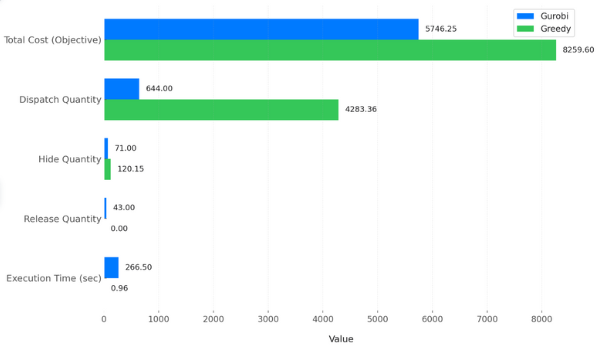
\includegraphics[width=textwidth]{Zhongzheng.png}
\caption{ZhongZheng District}
\label{Figure 1}
\end{figure}

\begin{figure}[H]
\centering
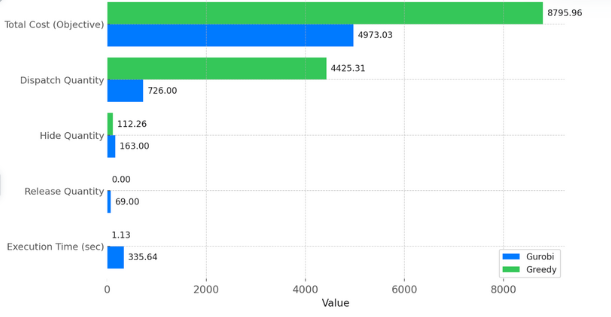
\includegraphics[width=textwidth]{Xinyi.png}
\caption{XinYi District}
\label{Figure 2}
\end{figure}

\begin{figure}[H]
\centering
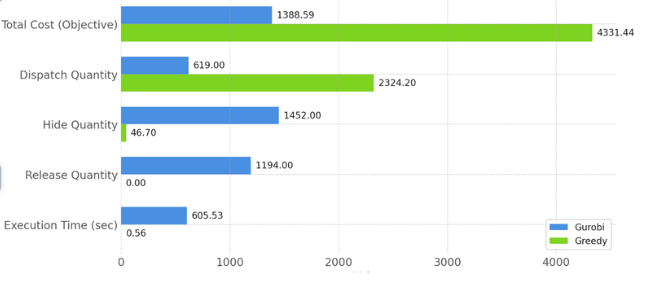
\includegraphics[width=textwidth]{Datong.png}
\caption{DaTong District}
\label{Figure 3}
\end{figure}

\begin{figure}[H]
\centering
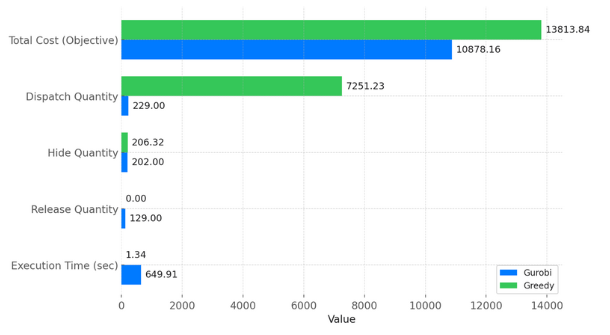
\includegraphics[width=textwidth]{Daan.png}
\caption{DaAn District}
\label{Figure 4}
\end{figure}

\section{Conclusions}

Abcde.

\vspace{0.5em}

\end{document}